\section{Key Missions and Turning Points}

\subsection{Robotic Luna, Ranger, and Surveyor}
Before any crew could land, both nations sent robotic scouts to study the Moon. The Soviet Luna program achieved a string of firsts, including the first impact on the lunar surface and the first images of its far side, expanding humanity's map of a world no one had yet touched.

American robotic missions followed a deliberate progression. Ranger probes returned close-up images as they crashed into the surface, while the Surveyor landers demonstrated soft landing and showed that the lunar soil could bear the weight of a spacecraft, easing fears that a lander might simply sink.

The robotic race had its own rhythm of failure and recovery. Early Rangers missed the Moon entirely or returned no pictures, and Luna probes fell silent in transit, yet each loss taught navigation, communication, and reliability lessons that the next attempt absorbed. By the mid-1960s both programs could hit a target a quarter of a million miles away with growing confidence.

Lunar Orbiter spacecraft then photographed the Moon systematically from orbit, producing the maps from which Apollo's landing sites were chosen. The candidate plains had to be smooth enough for a lander, well lit at the planned arrival time, and reachable with the fuel available, and only orbital photography could certify all three.

The Soviet robotic line continued even after the crewed race was lost. Luna 16 returned a soil sample by automated drill in 1970, and the Lunokhod rovers drove kilometers across the surface under remote control, achievements the Soviet press presented as proof that machines could do cheaply what Apollo did with risk. The argument was self-serving, but the engineering behind it was real.

Together these missions reduced risk. They mapped hazards, measured surface properties, and validated the navigation and landing techniques that crews would later depend on, turning the Moon from an unknown into a surveyed destination. \cite{siddiqi2010} \cite{nasa2019}

\subsection{Apollo 11 and lunar samples}
On 20 July 1969 Apollo 11's lunar module Eagle touched down in the Sea of Tranquility, and Neil Armstrong and Buzz Aldrin became the first humans to walk on another world. Hundreds of millions watched or listened as a goal set eight years earlier was fulfilled with months to spare.

The landing itself was a test of nerve as much as engineering. Program alarms from an overloaded guidance computer interrupted the descent, and Armstrong took semi-manual control to fly past a boulder field, setting down with roughly thirty seconds of fuel margin. The calm voice loop between Houston and the crew became one of the defining recordings of the century.

The crew did more than plant a flag. They deployed scientific instruments and collected about twenty-two kilograms of rock and soil, the first material ever returned from the Moon, which scientists would study for decades to understand the Moon's age and origin.

The samples rewrote lunar science. Laboratory analysis dated the basalts at more than three billion years old, revealed a chemistry consistent with a violent shared origin with Earth, and turned speculative questions about the Moon's birth into measurable ones. Five further landings would extend the collection to hundreds of kilograms from six distinct sites.

Getting there had taken a machine of unprecedented scale. The Saturn V stood taller than the Statue of Liberty, burned thirteen tons of propellant every second at liftoff, and flew thirteen times without a single launch failure, a reliability record that still astonishes engineers. Its development consumed years of test stands, failures, and redesigns that the public mostly never saw.

The flight was also a triumph of navigation and computing. The onboard guidance computer, built from early integrated circuits and woven core-rope memory, held less storage than a modern greeting card yet steered three men across a quarter of a million miles and back. Its priority-scheduling software, which kept the landing alive through those program alarms, became a foundational case study in real-time computing.

Apollo 11 marked the decisive moment of the race. The United States had achieved the most visible objective first, and while exploration continued, the central question of who would reach the Moon had been answered. \cite{nasa2019} \cite{chaikin1994} \cite{logsdon2010}

\begin{figure}[htbp]
\centering

\includegraphics[width=0.88\linewidth]{figures/ch04_lunar_surface.jpg}
\caption{Apollo 11 Lunar Module Eagle on the Moon surface.}
\label{fig:ch_apollo_11_lunar_module_eagle_on_}
\end{figure}

\begin{figure}[htbp]
\centering
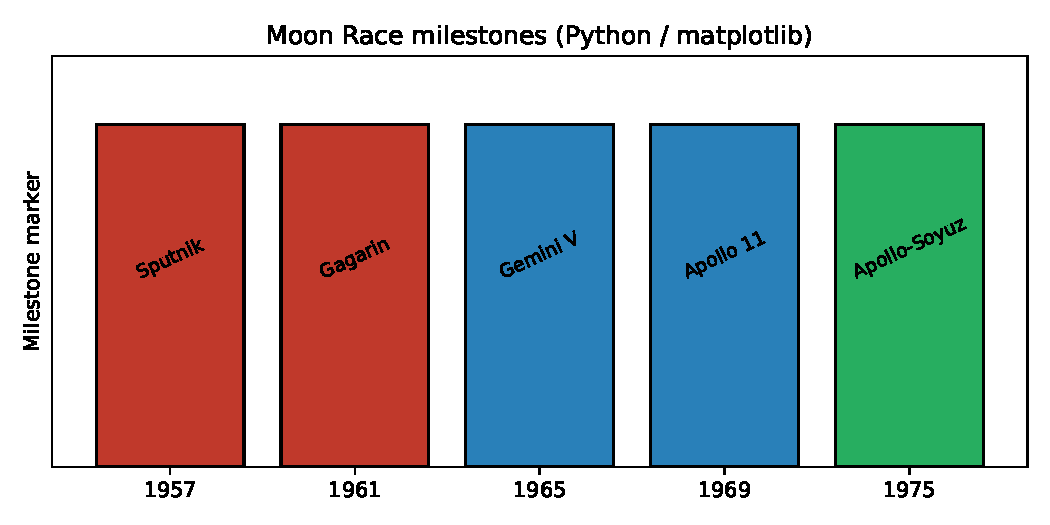
\includegraphics[width=0.92\linewidth]{figures/mission_timeline.pdf}
\caption{Moon Race milestones chart generated with Python (matplotlib).}
\label{fig:timeline}
\end{figure}

\bigskip
\begin{otherlanguage}{hebrew}
\subsection*{סיכום הפרק}

פרק זה סוקר משימות מפתח: גשושיות רובוטיות שמיפו את הירח, ולאחריהן נחיתת אפולו {\beginL 11\endL} שהביאה דגימות ראשונות מפני הירח.

\end{otherlanguage}

\clearpage
